\documentclass[a4paper]{article}


% import packages
\usepackage{graphicx}  % for \includegraphics with jpg,png,...
\usepackage[english,ngerman]{isodate, babel}  % ngerman: Neue Rechtschreibung
\usepackage{url}
\usepackage[dvipsnames]{xcolor}  % for \color
\usepackage{listings}  % source code support
\usepackage[T1]{fontenc}
\usepackage[utf8]{inputenc}
\usepackage{textcomp}  % support for symbols like €
\usepackage{lmodern}  % improve font
\usepackage{float}  % allow H option in \begin{figure}[H]
\usepackage{caption}
\usepackage{hyperref}
\usepackage[%
backend = biber,
sortlocale=de_DE,
natbib=true,
style = numeric,
autocite = inline
]{biblatex}
\addbibresource{references.bib}


% configure packages
\setlength{\columnsep}{8mm}

% redefine hyperref names
\addto\extrasngerman{
	\renewcommand{\sectionautorefname}{Kapitel}
	\renewcommand{\subsectionautorefname}{Abschnitt}
	\renewcommand{\subsubsectionautorefname}{Unterabschnitt}
}

\definecolor{codebg}{HTML}{eff0f1}
\lstset{
    backgroundcolor=\color{codebg},
    breaklines=true,
    tabsize=2,
    basicstyle=\small\ttfamily\bfseries,
    postbreak=\kern-5ex\mbox{\textcolor{gray}{$\hookrightarrow$}\space},
    numbers=left,
    numberstyle=\color{gray},
    showspaces=false,
    showstringspaces=false,
    tabsize=1,
    frame=single,
    rulecolor=\color{white},
    xleftmargin=3pt,
    xrightmargin=3pt,
}
% from https://github.com/cansik/kotlin-latex-listing
\lstdefinelanguage{Kotlin}{
    comment=[l]{//},
    commentstyle={\color{gray}\ttfamily},
    emph={delegate, filter, first, firstOrNull, forEach, lazy, map, mapNotNull, println, return@},
    emphstyle={\color{OrangeRed}},
    identifierstyle=\color{black},
    keywords={abstract, actual, as, as?, break, by, class, companion, continue, data, do, dynamic, else, enum, expect, false, final, for, fun, get, if, import, in, interface, internal, is, null, object, override, package, private, public, return, set, super, suspend, this, throw, true, try, typealias, val, var, vararg, when, where, while},
    keywordstyle={\color{NavyBlue}\bfseries},
    morecomment=[s]{/*}{*/},
    morestring=[b]",
    morestring=[s]{"""*}{*"""},
    ndkeywords={@Deprecated, @JvmField, @JvmName, @JvmOverloads, @JvmStatic, @JvmSynthetic, Array, Byte, Double, Float, Int, Integer, Iterable, Long, Runnable, Short, String},
    ndkeywordstyle={\color{BurntOrange}\bfseries},
    sensitive=true,
    stringstyle={\color{ForestGreen}\ttfamily},
}

\setlength{\parindent}{0cm}  % remove paragraph indentation
\setlength{\intextsep}{8pt}  % set space between two float objects

\raggedbottom  % move spacing produced by figures to the bottom of the page


\begin{document}

\title{\textbf{stock-simulator}}
\author{
    Jan Müller\\
    Jonas Thelemann\\
    Juri Lozowoj\\
    Lucas Held
}
\date{27. März 2020}
\maketitle

\pagebreak
\tableofcontents
\pagebreak

\begin{lstlisting}[caption={example kotlin code}, captionpos=b, label={lst:example}, language=Kotlin]
private suspend fun StockbrotQuote.executeSellOrder(quote: Quote) {
    val depotQuote = accountRepository.depotQuoteBySymbol(id) ?: return
    if (quote.latestPrice >= minimumSellPrice) {
        val amount = depotQuote.amount
        Timber.i("Bot is selling $amount for ${quote.latestPrice}")
        accountRepository.sell(quote, amount)
    }
}
\end{lstlisting}

\begin{figure}[H]
    \centering
    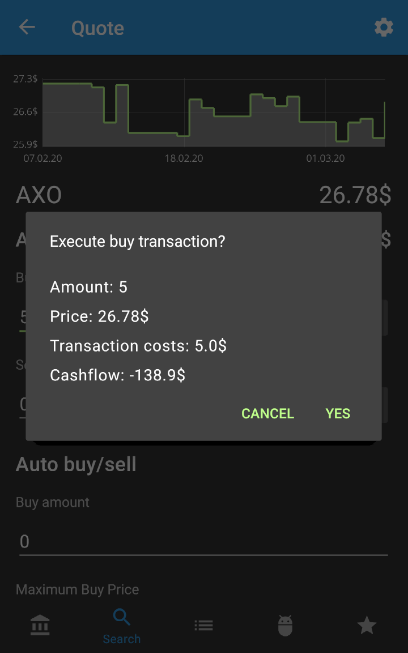
\includegraphics[height=10cm,keepaspectratio]{./images/quote_buy_confirmation_dialog.png}
    \caption{example image}
    \label{fig:example}
\end{figure}

\pagebreak


\section{Einleitung}
\label{sec:introduction}
% Gute Einleitung ins Thema (was war die Aufgabe, etc.)
Aufgabe der Veranstaltung "`Code-Camp Context-Awareness 1"' war die Entwickelung eines Börsensimulator Spiels für Android Smartphones. Dabei stellte das Verwenden von echten Aktienkursen, mit aktuellen Daten, eine wichtige Anforderung an das Spiel dar. Diese Daten sollten als Basis für alle weiteren Funktionen dienen. Mithilfe des zur Verfügung stehenden Spielgeldes soll der Benutzer die Möglichkeit haben, Aktien oder Kryptowährungen zu kaufen. Um das Kaufen von bestimmten Aktien und Kryptowährungen zu ermöglichen, wurde eine Suchfunktion gefordert, welche die verfügbaren Elemente filtert und anzeigt. Um das Budget immer im Blick zu behalten, muss es Depotübersicht, sowie eine Anzeige für den aktuellen Kontostand und dessen Verlauf geben. Eine Historie soll die Käufe und Verkäufe in der Vergangenheit darstellen. Als Darstellungsform der Kurse und des Kontoverlaufs sind Graphen zu wählen. Wie auf gängigen Tradingplatformen soll auch der Simulator mit jedem Kauf- oder Verkauf Transaktionskosten berechnen. Ein Bot soll das Traden übernehmen, falls dies vom Benutzer gewünscht wird. Entsprechende Zielwerte sollen für jede Aktie oder Kryptowährung anpassbar sein. Damit der Benutzer die Möglichkeit hat, das Spiel neu zu beginnen, muss die Anwendung eine Option bieten, den Spielstand zurückzusetzen. Zusätzlich zu den bisher genannten Hauptfeatures, wird mindestens ein Zusatzfeature gefordert, welches eine nützliche Erweiterung für die Anwendung darstellt. Ziel des Spiels ist es, das Startkapital im Laufe der Zeit möglichst stark zu vermehren.


\section{Technische Details}
\label{sec:technologies}
TODO


\subsection{Architektur}
\label{subsec:technologies:architecture}
% App Architektur (Welches Pattern habt ihr benutzt? MVVM? Livedata?) Was ist das und warum ist das cool?
% Schwierigkeiten und wie ihr sie gelöst habt
Die App-Architektur folgt offiziellen Empfehlungen\autocite{google_recommendations} und basiert auf einer \textit{Activity} sowie dem \textit{Model-View-ViewModel-Pattern} (MVVM).
Bei diesem Entwurfsmuster werden die Präsentation der Benutzeroberfläche und die angebundene Logik voneinander getrennt.

Dazu verwenden Benutzeroberflächen \textit{Databinding}, um von \textit{ViewModels} bereitgestellte Daten anzuzeigen.
Der dafür notwendige Quelltext wird automatisch generiert, wodurch Fehleranfälligkeit reduziert und Entwicklung beschleunigt werden.

\textit{ViewModels} sind für das Verhalten von Benutzeroberflächen verantwortlich und beziehen ihre Daten wiederum aus \textit{Models}, welche in Form von \textit{Repositories} implementiert sind.

\textit{Repositories} dienen als \textit{Single Point of Truth}, wodurch fehlerhafte oder inkonsistente Datenbestände vermieden werden.
Sie sind an die interne Datenbank (siehe \autoref{subsubsec:technologies:bibs:room}) sowie verschiedene Netzwerkquellen (siehe \autoref{subsec:technologies:apis}) angebunden.

%unfertig, sehr raw

\subsection{APIs}
\label{subsec:technologies:apis}
TODO


\subsubsection{IEX Cloud}
\label{subsubsec:technologies:apis:iex}
% https://iexcloud.io/
TODO


\subsubsection{CoinGecko}
\label{subsubsec:technologies:apis:coingecko}
% https://www.coingecko.com/
TODO


\subsection{Bibliotheken}
\label{subsec:technologies:bibs}
TODO


\subsubsection{Android Jetpack}
\label{subsubsec:technologies:bibs:jetpack}
% https://developer.android.com/jetpack/
TODO


\subsubsection{Moshi}
\label{subsubsec:technologies:bibs:moshi}
% https://github.com/square/moshi
TODO


\subsubsection{Room}
\label{subsubsec:technologies:bibs:room}
% https://developer.android.com/jetpack/androidx/releases/room
TODO


\subsubsection{Retrofit}
\label{subsubsec:technologies:bibs:retrofit}
% https://github.com/square/retrofit
TODO


\section{Funktionalität}
\label{sec:functionality}
% Welche Features habt ihr gebaut?
% Welche Screens habt ihr gebaut?
% Warum sehen die Screens so aus? (warum ist button X an Position Y) / was habt ihr euch dabei gedacht?
Im Folgenden werden die 


\subsection{Navigation}
\label{subsec:functionality:navigation}
Über die \textit{Bottom Navigation}\autocite{bottom_navigation} können Nutzer zwischen den Hauptfeatures Account, Suche, Transaktionsverlauf, Stockbrot und Errungenschaften wechseln.
Diese Art der Navigation wurde gewählt, da sie modernen Designempfehlungen entspricht und bessere Kompatibilität mit Android 10 Gesten aufweist als beispielsweise ein \textit{Hamburger Menü}.


\subsection{Account}
\label{subsec:functionality:account}
TODO


\subsection{Suche}
\label{subsec:functionality:search}
Das Suchen von Aktien und Kryptowährungen nach Name und Symbol ist im Search-Screen möglich.
Zudem können Nutzer dort auswählen, ob sie nur Aktien oder Kryptowährungen sehen möchten.

\autoref{fig:functionality:search:full} zeigt den Aufbau dieses Screens.
Das Eingabefeld für Suchanfragen und die Dropdown-Liste zum Filtern befinden sich am oberen Bildschirmrand.
Darunter werden Suchergebnisse in einem scrollbaren Raster angezeigt.
Diese Aktualisieren sich automatisch, sobald sich ein Suchkriterium verändert.
Dadurch ist es möglich auf Nutzereingaben unmittelbar zu reagieren und Ergebnisse schnell anzuzeigen.
Während eine Suche stattfindet wird ein Fortschritts\-indikator angezeigt, um Nutzer über den aktuellen Zustand zu informieren.

Durch Klicken auf ein Suchergebnis können Nutzer zur Detailansicht dieses Anlageguts navigieren (siehe \autoref{subsec:functionality:quote}).

\begin{figure}[H]
	\centering
	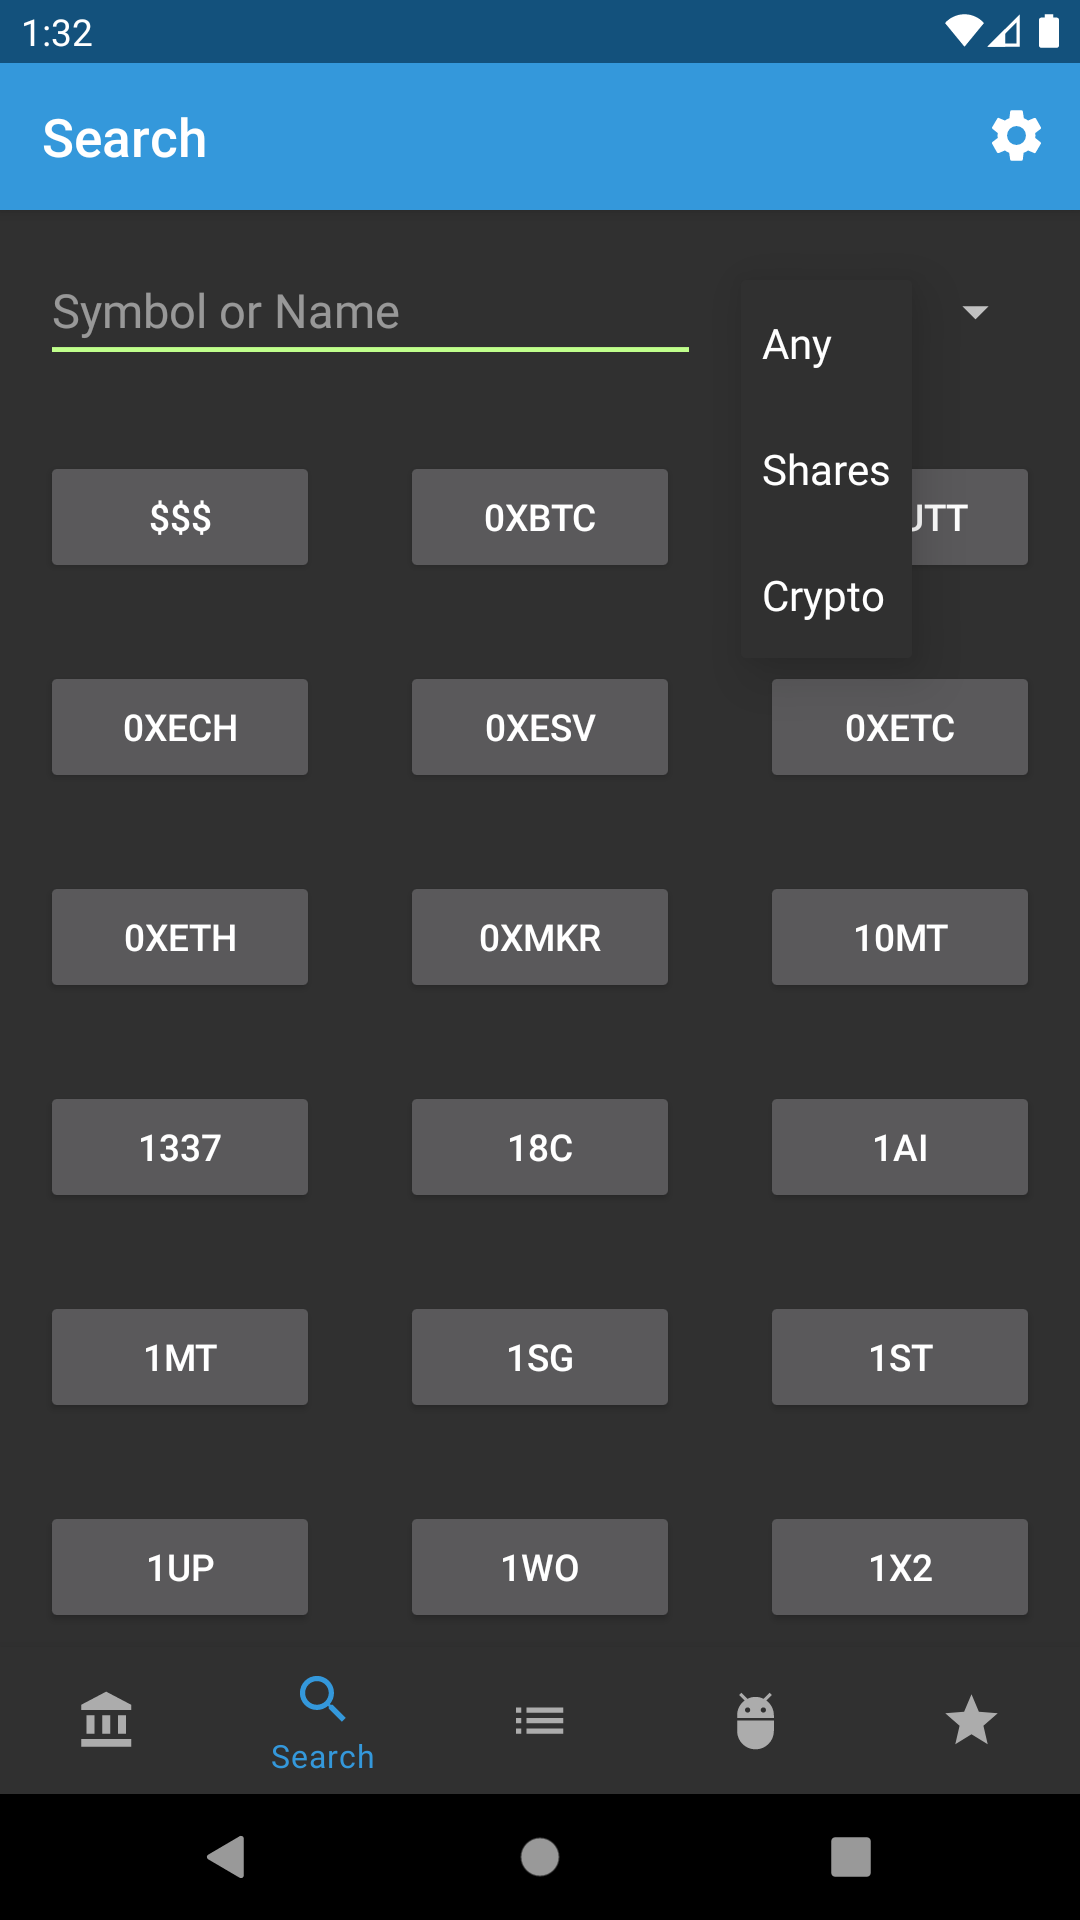
\includegraphics[height=7cm,keepaspectratio]{./images/search_type.png}
	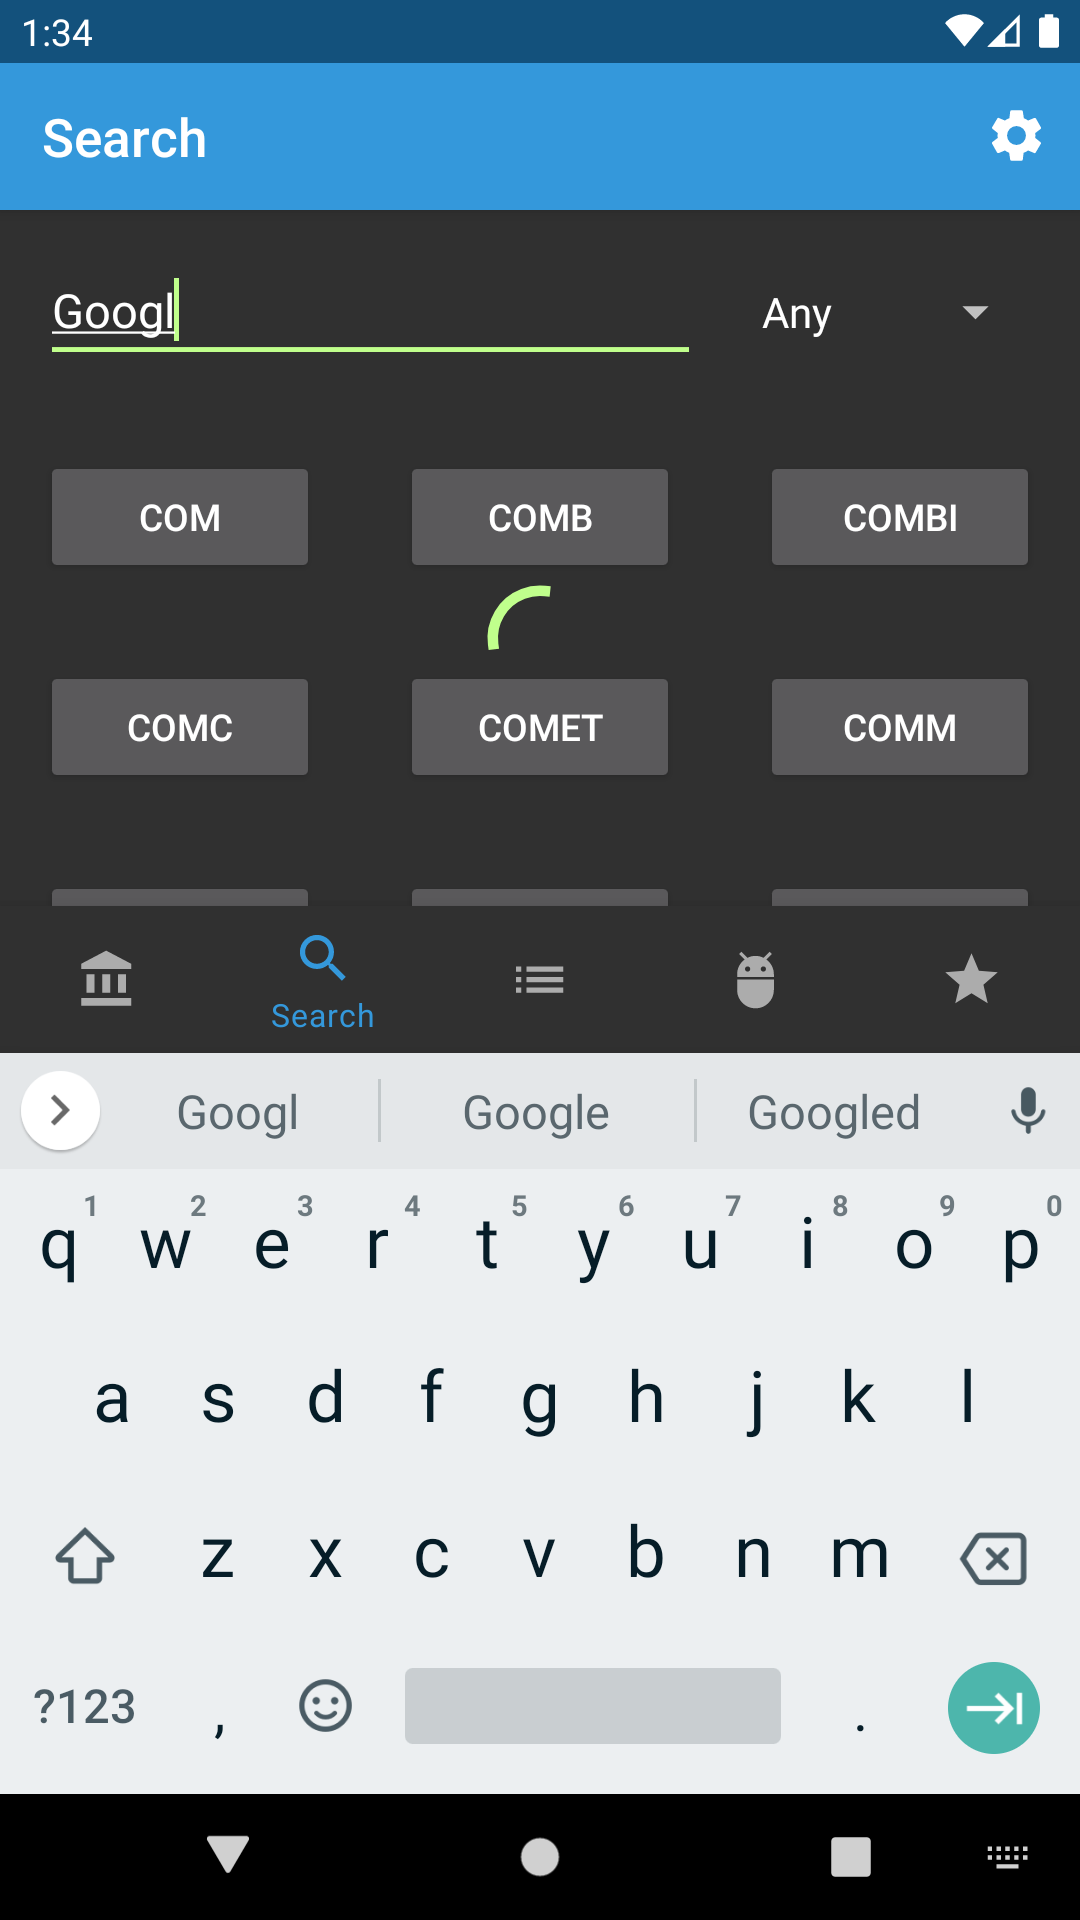
\includegraphics[height=7cm,keepaspectratio]{./images/search_loading.png}
	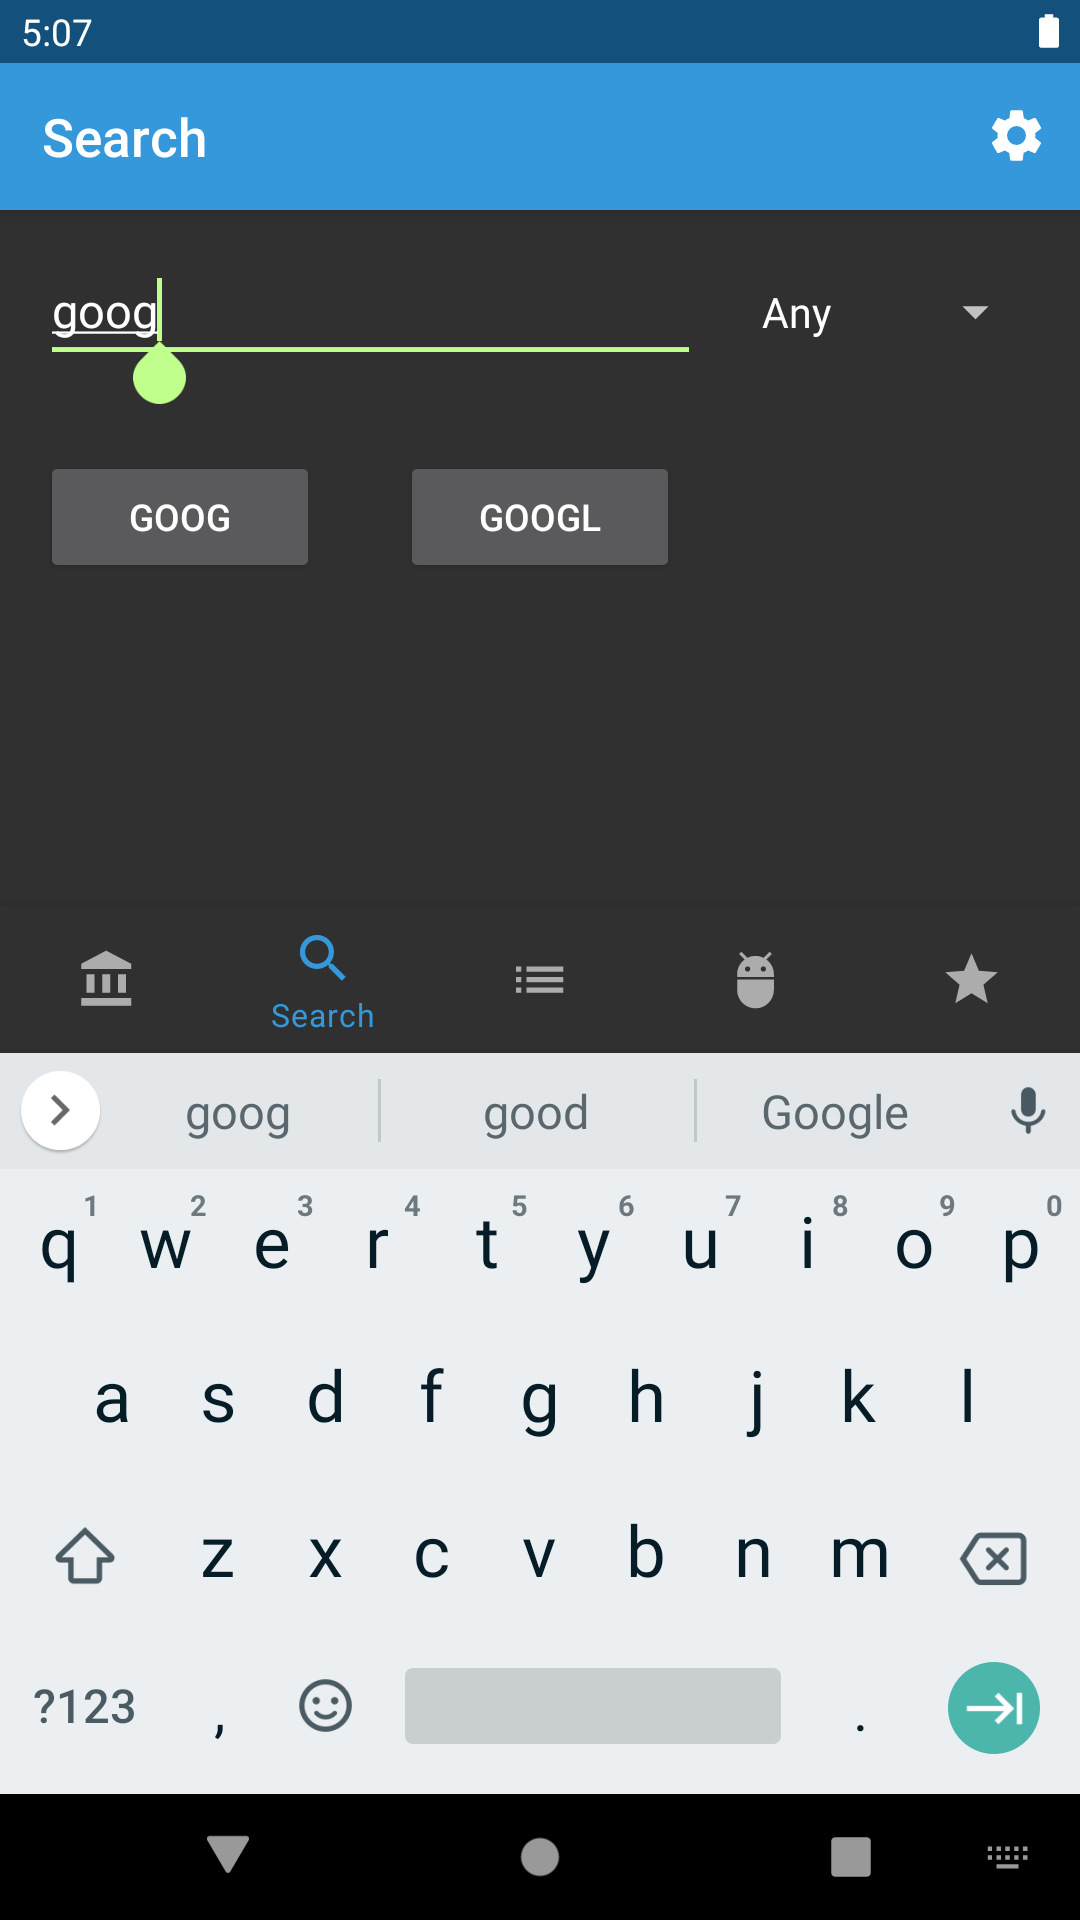
\includegraphics[height=7cm,keepaspectratio]{./images/search_done.png}
	\caption{Suche}
	\label{fig:functionality:search:full}
\end{figure}


\subsection{Transaktionsverlauf}
\label{subsec:functionality:history}
TODO


\subsection{Stockbrot}
\label{subsec:functionality:stockbrot}
TODO


\subsection{Errungenschaften}
\label{subsec:functionality:achievements}
TODO


\subsection{Detailansicht}
\label{subsec:functionality:quote}
TODO


\subsection{News}
\label{subsec:functionality:news}
TODO


\subsection{Einstellungen}
\label{subsec:functionality:settings}
TODO


\section{Teamwork}
\label{sec:teamwork}
TODO


\section{Zusammenfassung}
\label{sec:summary}
TODO


\section{Fazit}
\label{sec:conclusion}
TODO


\section{Ausblick}
\label{sec:outlook}
% was kann man noch machen, was habt ihr nicht geschafft,..
TODO


\printbibliography[title={Referenzen}]


\end{document}
